\section{Non-crossing Partitions}

\begin{definition}[Non-crossing Partition]
    A \emph{non-crossing partition} of a \emph{totally
    ordered} set $E$ is
    a set partition $P = \{E_1, E_2, \ldots, E_k\}$ such that
    if $a, c \in E_i$, $b, d \in E_j$, and $i \neq j$, then
    we do \emph{not} have $a < b < c < d$, nor $a > b > c > d$.\\
    We denote by $\mathcal{NC}_n$ the set of non-crossing partitions
    of $\{1, 2, \ldots, n\}$.
    $$\mathcal{NC} = \bigcup_{n > 0}{\mathcal{NC}_n}$$
\end{definition}

From this point, we assume that every partition $P = \{B_1, \ldots, B_l\}$
is \emph{sorted} such that :\\
\begin{itemize*}
    \item For each block $B_i = \{b_1, \ldots, b_k\} \in P$,
        $b_1 < \ldots < b_k$\\
    \item $min (B_1) < \ldots < min (B_k)$\\
\end{itemize*}

\begin{notation}
    $[n] = \{1, 2, \ldots, n\}$
\end{notation}

\begin{example}[$E = \lbrack 6 \rbrack $]
    \begin{align*}
        &P_1 = \{\{1, 2, 5\}, \{3, 4\}, \{6\}\} \in \mathcal{NC}_6\\
        &P_2 = \{\{1, 2, 4\}, \{3, 5\}, \{6\}\} \notin \mathcal{NC}_6
    \end{align*}
\end{example}

\begin{theorem}
    Let $nc_n$ be the cardinal of $\mathcal{NC}_n$.
    We have $$nc_n = \frac{1}{n + 1} \binom{2n}{n}$$
    which is again the $n^{th}$ Catalan number
    $Cat(n)$.
\end{theorem}

\begin{example}[$n = 1, 2, 3$]
    ~\\
    \begin{itemize*}
        \item $n = 1$ \  $:$ \  $nc_1 = 1$\\
        \subitem $\{\{1\}\}$\\
        \item $n = 2$ \  $:$ \  $nc_2 = 2$\\
        \subitem $\{\{1, 2\}\}$
        \subitem $\{\{1\}, \{2\}\}$\\
        \item $n = 3$ \  $:$ \  $nc_3 = 5$\\
        \subitem $\{\{1, 2, 3\}\}$
        \subitem $\{\{1\}, \{2, 3\}\}$
        \subitem $\{\{1, 3\}, \{2\}\}$
        \subitem $\{\{1, 2\}, \{3\}\}$
        \subitem $\{\{1\}, \{2\}, \{3\}\}$\\
    \end{itemize*}
\end{example}

\begin{prop}
    This means we can create a \emph{bijection} between
    $\mathcal{PF'}_n$ and $\mathcal{NC}_n$.
\end{prop}

\begin{proof}
    ~\\
\begin{itemize}
    \item $\mathcal{NC}_n \to \mathcal{PF'}_n$ :
    For each block $B$ in the non-crossing partition, take
    $i = min (B)$, and let $k_i = size (B)$.\\
    $k_i = 0$ if $i$ is not the minimum of a block.\\
    The corresponding parking function is
    $(\underbrace{1, \ldots, 1}_{k_1}, \underbrace{2, \ldots,
    2}_{k_2}, \ldots, \underbrace{n, \ldots, n}_{k_n})$.\\
    \item $\mathcal{PF'}_n \to \mathcal{NC}_n$ :
    For each $i$ in $[n]$, if $i$ appears $n_i$ times in the
    parking function, $B_i$ will be of size $n_i$ with minimum
    element $i$.
    There is a unique set partition $\displaystyle P = \bigcup_{i}{B_i}$
    of $[n]$ respecting these conditions that is non-crossing :
    for each minimum $i$ in \emph{decreasing order}, add
    the $n_i$ first free elements of
    $[i+1, i+2, \ldots, n, 1, \ldots, i-1]$ to $B_i$.
\end{itemize}
\end{proof}

\begin{example}[$n = 6$]
    \begin{align*}
        &P = \{\{1, 2, 5\}, \{3, 4\}, \{6\}\}
        &f = (1, 1, 1, 3, 3, 6)\\
    \end{align*}
\end{example}

\begin{cor}
    A non-crossing partition can be represented by the minimums
    and sizes of its blocks.
\end{cor}

\begin{example}
    $\{\{1, 2, 5\}, \{3, 4\}, \{6\}\}$ can be represented by
    the following dictionnary :\\
    \begin{itemize*}
        \item 1 : 3\\
        \item 3 : 2\\
        \item 6 : 1\\
    \end{itemize*}
\end{example}

A non-crossing partition of $[n]$ can be represented graphically
on a regular $n$-vertices polygon, with vertices labeled from $1$
to $n$ clockwise. We then represent each block $B = \{b_1, \ldots, b_k\}$
by the convex hull of $\{b_1, \ldots, b_k\}$.\\

\begin{example}[$P = \{\{1, 2, 5\}, \{3, 4\}, \{6\}\}$]
    ~\\
    \begin{center}
        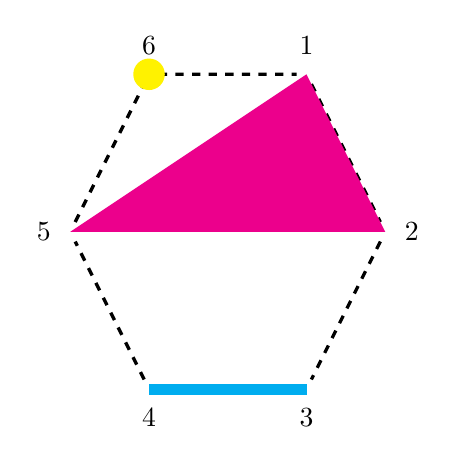
\begin{tikzpicture}[scale=1]
            \node [label = above : {$1$}] (1)
                at (4,5) {};
            \node [label = right : {$2$}] (2)
                at (5,3) {};
            \node [label = below : {$3$}] (3)
                at (4,1) {};
            \node [label = below : {$4$}] (4)
                at (2,1) {};
            \node [label = left : {$5$}]  (5)
                at (1,3) {};
            \node [label = above : {$6$}] (6)
                at (2,5) {};
            \draw [dashed][very thick]
            (1) -- (2) -- (3) -- (4)
                -- (5) -- (6) -- (1);
            \fill [color = magenta] (4,5) -- (5,3)
                -- (1,3) -- cycle;
            \draw [color = cyan][line width = 4pt] 
                (4,1) -- (2,1);
            \fill [color=yellow] (2,5) circle (0.2);
          \end{tikzpicture}
    \end{center}
    Thus non-crossing meaning the hulls are
    \emph{disjoint}.\\
\end{example}

\begin{example}[Counter-example : $P = \{\{1, 5, 2\},
    \{3, 6\}, \{4\}\}$]
    ~\\
    \begin{center}
        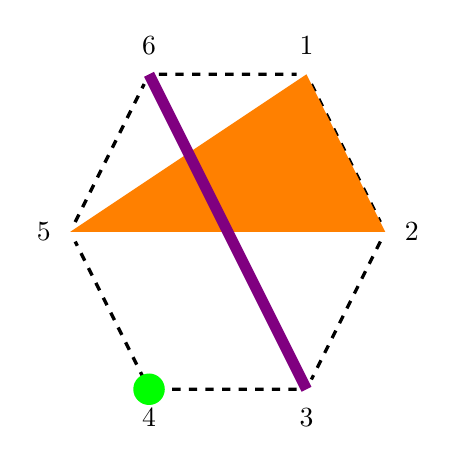
\begin{tikzpicture}[scale=1]
            \node [label = above : {$1$}] (1)
                at (4,5) {};
            \node [label = right : {$2$}] (2)
                at (5,3) {};
            \node [label = below : {$3$}] (3)
                at (4,1) {};
            \node [label = below : {$4$}] (4)
                at (2,1) {};
            \node [label = left : {$5$}]  (5)
                at (1,3) {};
            \node [label = above : {$6$}] (6)
                at (2,5) {};
            \draw [dashed][very thick]
            (1) -- (2) -- (3) -- (4)
                -- (5) -- (6) -- (1);
            \fill [color = orange] (4,5) -- (5,3)
                -- (1,3) -- cycle;
            \draw [color = violet][line width = 4pt] 
                (4,1) -- (2,5);
            \fill [color=green] (2,1) circle (0.2);
          \end{tikzpicture}
    \end{center}
    This partition is \emph{not} non-crossing, as the
    convex hulls of $\{1, 2, 5\}$ and $\{3, 6\}$ are
    \emph{not} disjoint.
\end{example}

\subsection{The non-crossing partitions poset}

\begin{definition}[$\succ$]
    We say that $P$ covers $Q$, written $P \succ Q$,
    if $\exists B_i, B_j \in P$ such that
    $Q = P - \{B_i, B_j\} \cup \{B_i \cup B_j\}$    
\end{definition}

\begin{example}
    $\{\{1, 6\}, \{2, 3\}, \{4, 5\}\} \succ
    \{\{1, 2, 3, 6\}, \{4, 5\}\}$\\
    \begin{itemize*}
        \item $B_i = \{1, 6\}$\\
        \item $B_j = \{2, 3\}$\\
    \end{itemize*}
\end{example}

\begin{prop}
    This covering relation defines the \emph{poset}
    of $\mathcal{NC}_n$.
    We denote by $\mathcal{NCC}_n$ the set of
    \emph{maximal chains} in the poset of $\mathcal{NC}_n$.\\
    $$\mathcal{NCC} = \bigcup_{n > 0}{\mathcal{NCC}_n}$$
\end{prop}

\begin{rem}
    The bottom element of this poset is $\{\{1, \ldots, n\}\}$,
    and the top element is $\{\{1\}, \ldots, \{n\}\}$.
\end{rem}

\begin{theorem}
    Let $ncc_n$ be the cardinal of $\mathcal{NCC}_n$.
    We have $$ncc_n = n^{n - 2}$$.
\end{theorem}

\begin{example}[The poset of $\mathcal{NC}_4$]
    ~\\
    To shorten labels, we represent $\{\{1\}, \{2, 3\},
    \{4\}\}$ by $1|23|4$. \\

    \begin{center}
        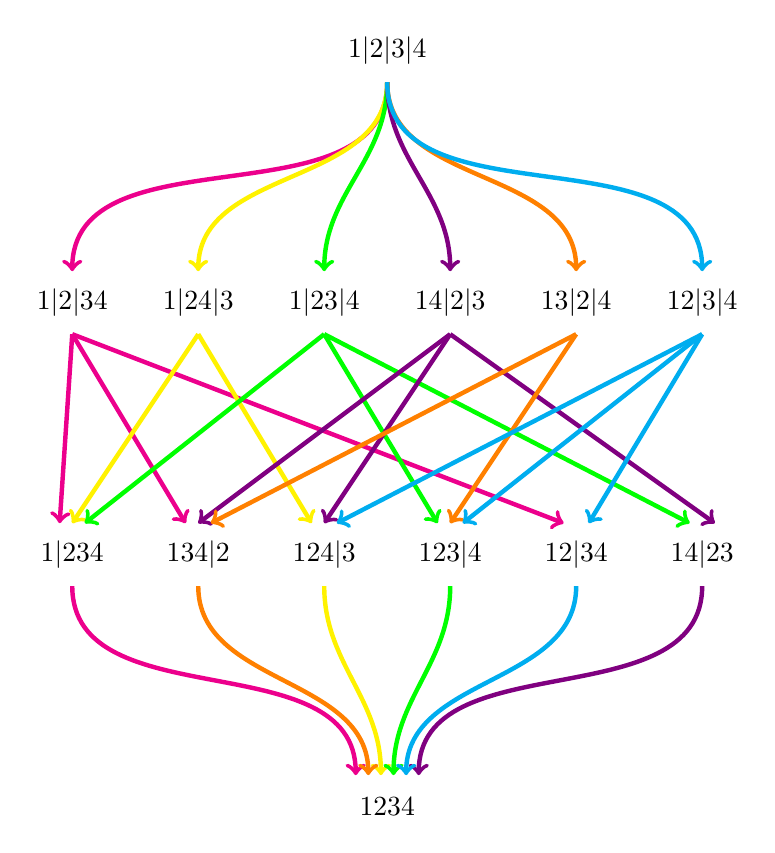
\begin{tikzpicture}[scale = 0.8]
            \node (0)  at (0,0)  {$1234$};
            \node (1)  at (-5,4) {$1|234$};
            \node (2)  at (-3,4) {$134|2$};
            \node (3)  at (-1,4) {$124|3$};
            \node (4)  at (1,4)  {$123|4$};
            \node (5)  at (3,4)  {$12|34$};
            \node (6)  at (5,4)  {$14|23$};
            \node (7)  at (-5,8) {$1|2|34$};
            \node (8)  at (-3,8) {$1|24|3$};
            \node (9)  at (-1,8) {$1|23|4$};
            \node (10) at (1,8)  {$14|2|3$};
            \node (11) at (3,8)  {$13|2|4$};
            \node (12) at (5,8)  {$12|3|4$};
            \node (13) at (0,12) {$1|2|3|4$};
        
            \draw [->][out=-90,in=90, ultra thick] 
                [color=magenta](0,11.5) to (-5,8.5);
            \draw [->][color=magenta, ultra thick]
                (-5,7.5) to (-5.2,4.5);
            \draw [->][color=magenta, ultra thick]
                (-5,7.5) to (-3.2,4.5); 
            \draw [->][color=magenta, ultra thick]
                (-5,7.5) to (2.8,4.5);
            \draw [->][out=-90,in=90, ultra thick] 
                [color=magenta](-5,3.5) to (-0.5,0.5);
        
            \draw [->][out=-90,in=90, ultra thick]
                [color=yellow] (0,11.5) to (-3,8.5);
            \draw [->][color=yellow, ultra thick]
                (-3,7.5) to (-5,4.5);
            \draw [->][color=yellow, ultra thick]
                (-3,7.5) to (-1.2,4.5);
            \draw [->][out=-90,in=90, ultra thick] 
                [color=yellow](-1,3.5) to (-0.1,0.5);
            
            \draw [->][out=-90,in=90, ultra thick]
                [color=green](0,11.5) to (-1,8.5);
            \draw [->][color=green, ultra thick]
                (-1,7.5) to (-4.8,4.5);
            \draw [->][color=green, ultra thick]
                (-1,7.5) to (0.8,4.5);
            \draw [->][color=green, ultra thick]
                (-1,7.5) to (4.8,4.5);
            \draw [->][out=-90,in=90, ultra thick] 
                [color=green](1,3.5) to (0.1,0.5);
        
            \draw [->][out=-90,in=90, ultra thick]
                [color=violet](0,11.5) to (1,8.5);
            \draw [->][color=violet, ultra thick]
                (1,7.5) to (-3,4.5);
            \draw [->][color=violet, ultra thick]
                (1,7.5) to (-1,4.5);
            \draw [->][color=violet, ultra thick]
                (1,7.5) to (5.2,4.5);
            \draw [->][out=-90,in=90, ultra thick] 
                [color=violet](5,3.5) to (0.5,0.5);
        
            \draw [->][out=-90,in=90, ultra thick]
                [color=orange](0,11.5) to (3,8.5);
            \draw [->][color=orange, ultra thick]
                (3,7.5) to (-2.8,4.5);
            \draw [->][color=orange, ultra thick]
                (3,7.5) to (1,4.5);
            \draw [->][out=-90,in=90, ultra thick] 
                [color=orange](-3,3.5) to (-0.3,0.5);
        
            \draw [->][out=-90,in=90, ultra thick]
                [color=cyan](0,11.5) to (5,8.5);
            \draw [->][color=cyan, ultra thick]
                (5,7.5) to (-0.8,4.5);
            \draw [->][color=cyan, ultra thick]
                (5,7.5) to (1.2,4.5);
            \draw [->][color=cyan, ultra thick]
                (5,7.5) to (3.2,4.5);
            \draw [->][out=-90,in=90, ultra thick] 
                [color=cyan](3,3.5) to (0.3,0.5);
        
        \end{tikzpicture}
        ~\\
        ~\\
        There are $4^2 = 16$ different maximal chains,
        and $\frac {1}{5} \binom{8}{4} = \frac{70}{5} = 14$
        elements in this poset.
    \end{center}
\end{example}



\subsection{Kreweras complement}

\begin{definition}[Associated Permutation]
    The \emph{permutation} $\sigma$ associated to a non-crossing
    partition has a cycle $(b_1, \ldots, b_k)$ for each block
    $B = \{b_1, \ldots, b_k\}$ of the partition.
\end{definition}

\begin{example}
    The permutation associated to $\{\{1, 2, 5\}, \{3, 4\}, \{6\}\}$
    is $(1\ 2\ 5)\ (3\ 4)\ (6) = 254316$.
\end{example}

\begin{definition}[Kreweras Complement]
    The \emph{Kreweras complement} $K (P)$ of a non-crossing
    partition $P$ is defined as follows :\\
    \begin{itemize*}
        \item Let $\sigma$ be the permutation associated to $P$\\
        \item Let $\pi$ be the permutation $(n\ n-1\ n-2\
        \ldots\ 3\ 2\ 1) = n123 \ldots n-1$\\
        \item $K (P)$ is the \emph{non-crossing partition}
        associated to $\pi \sigma$.\\
    \end{itemize*}
\end{definition}

\begin{example}[$P = \{\{1, 2, 5\}, \{3, 4\}, \{6\}\}$]
    ~\\
    \begin{itemize*}
        \item $\sigma = (1\ 2\ 5)\ (3\ 4)\ (6) = 254316$\\
        \item $\pi = (6\ 5\ 4\ 3\ 2\ 1) = 612345$\\
        \item $\pi \sigma = 143265 = (1)\ (2\ 4)\ (3)\ (5\ 6)$\\
        \item $K(P) = \{\{1\},\{2, 4\}, \{3\}, \{5, 6\}\}$\\
    \end{itemize*}
\end{example}

\begin{prop}[Kreweras minimums]
        Let $P = \{B_1, \ldots, B_k\}$ be a non-crossing partition.
        Let $K (P) = \{B'_1, \ldots, B'_l\}$ be its Kreweras complement.
        Then $$\bigcup_{1 \leq i \leq l}{min (B'_i)} =
        B_1 \cup \bigcup_{1 < j \leq k}{B_i - {max (B_i)}}$$\\
\end{prop}

\begin{example}[$P = \{\{1, 2, 5\}, \{3, 4\}, \{6\}\}$]
    ~\\
    \begin{itemize}
        \item $K (P) = \{\{1\},\{2, 4\}, \{3\}, \{5, 6\}\}$
        \item $\bigcup{min (B'_i)} = \{1, 2, 3, 5\}$
        \item $B_1\ \cup\ \bigcup{B_i - {max (B_i)}}
        = \{1, 2, 5\} \cup \{3, 4\} - \{4\} \cup \{6\} - \{6\}
        = \{1, 2, 5\} \cup \{3\} \cup \emptyset = \{1, 2, 3, 5\}$\\
    \end{itemize}
\end{example}

\begin{notation}
    $B_{[i]} = $ block containing $i$.
\end{notation}

\begin{prop}[Kreweras block sizes]
    Let $P = \{B_1, \ldots, B_k\}$ be a non-crossing partition.
    Let $K (P) = \{B'_1, \ldots, B'_l\}$ be its Kreweras complement.
    Then the size of the block $B'_i$ is defined as follows :
    \begin{itemize}
        \item Let $m_i$ be the the $i^{th}$ minimum of $K (P)$
        \item Define a \emph{transition} $\phi (e)$ as 
            \subitem Let $j = e + 1$ (or $1$ if $e = n$)
            \subitem $\phi(e) = max (B_{[j]})$
        \item The size of $B'_i$ is $k_{min}$ such that
        $k_{min} = min \{k > 0\ |\ \phi^k (m_i) \in B_{[m_i]}\}$.\\
    \end{itemize}
\end{prop}

\begin{example}[$P = \{\{1, 2, 5\}, \{3, 4\}, \{6\}\}$]
    ~\\
    \begin{itemize}
        \item $mins = \{1, 2, 3, 5\}$
        \item $m_1 = 1$
            \subitem $B_{[1]} = B_1$
            \subitem $max (B_{[2]} = max (B_1) = 5$
            \subitem The size for $m_1$ is $1$.
        \item $m_2$
            \subitem $B_{[2]} = B_1$
            \subitem $max (B_{[3]}) = max (B_2) = 4$
            \subitem $max (B_{[5]}) = max (B_1) = 5$
            \subitem The size for $m_2$ is $2$.
        \item $m_3 = 3$
            \subitem $B_{[3]} = B_2$
            \subitem $max (B_{[4]}) = max (B_2) = 4$
            \subitem The size for $m_3$ is $1$.
        \item $m_4 = 5$
            \subitem $B_{[5]} = B_1$
            \subitem $max (B_{[6]}) = max (B_3) = 6$
            \subitem $max (B_{[1]}) = max (B_1) = 5$
            \subitem The size for $m_4$ is $2$.
    \end{itemize}
\end{example}

\begin{definition}[Mutually Non-crossing Partitions]
    2 partitions $P$ and $Q$ are said
    \emph{mutually non-crossing} if :\\
    \begin{itemize*}
        \item P is non-crossing\\
        \item Q is non-crossing\\
        \item For every block $B_i$ of $P$ and every
        block $B_j$ of $Q$, if $a,c \in B_i$ and
        $b, d \in B_j$, then we can \emph{not} have
        $a < b < c < d$, nor $a > b > c > d$.
    \end{itemize*}    
\end{definition}

\begin{example}[$P = \{\{1, 2\},\{3, 6\},\ \{4, 5\}\},
    Q = \{\{1, 6\}, \{2\}, \{3, 4\}, \{5\}\}$]
    ~\\
    \begin{center}
        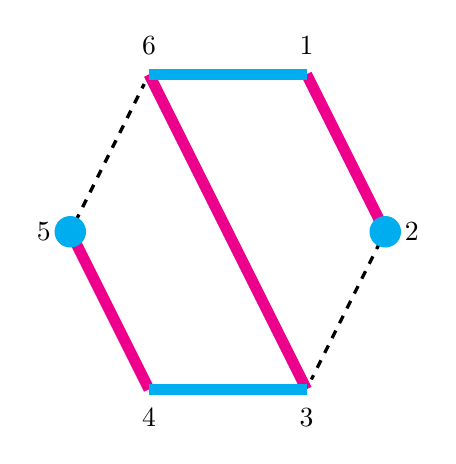
\begin{tikzpicture}[scale=1]
            \node [label = above : {$1$}] (1)
                at (4,5) {};
            \node [label = right : {$2$}] (2)
                at (5,3) {};
            \node [label = below : {$3$}] (3)
                at (4,1) {};
            \node [label = below : {$4$}] (4)
                at (2,1) {};
            \node [label = left : {$5$}]  (5)
                at (1,3) {};
            \node [label = above : {$6$}] (6)
                at (2,5) {};
            \draw [dashed][very thick]
            (1) -- (2) -- (3) -- (4)
                -- (5) -- (6) -- (1);
            \draw [color = magenta][line width = 4pt] 
                (4,5) -- (5,3);
            \draw [color = magenta][line width = 4pt] 
                (4,1) -- (2,5);
            \draw [color = magenta][line width = 4pt] 
                (2,1) -- (1,3);
            \draw [color = cyan][line width = 4pt] 
                (4,5) -- (2,5);                
            \draw [color = cyan][line width = 4pt] 
                (4,1) -- (2,1);
            \fill [color=cyan] (5,3) circle (0.2);
            \fill [color=cyan] (1,3) circle (0.2);
          \end{tikzpicture}
    \end{center}
\end{example}

\begin{example}[Counter-example : $P = \{\{1, 2\},
    \{3, 6\},\ \{4, 5\}\},
    Q = \{\{1, 6\}, \{2, 5\}, \{3, 4\}\}$]
    ~\\
    \begin{center}
        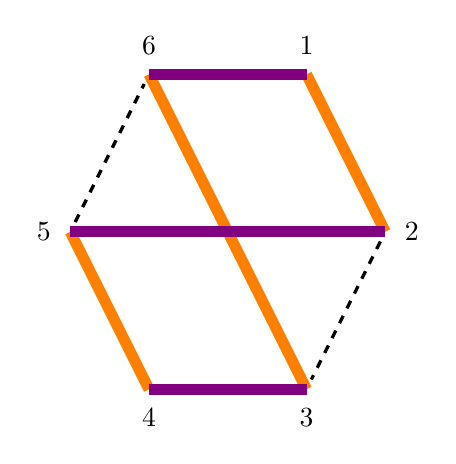
\begin{tikzpicture}[scale=1]
            \node [label = above : {$1$}] (1)
                at (4,5) {};
            \node [label = right : {$2$}] (2)
                at (5,3) {};
            \node [label = below : {$3$}] (3)
                at (4,1) {};
            \node [label = below : {$4$}] (4)
                at (2,1) {};
            \node [label = left : {$5$}]  (5)
                at (1,3) {};
            \node [label = above : {$6$}] (6)
                at (2,5) {};
            \draw [dashed][very thick]
            (1) -- (2) -- (3) -- (4)
                -- (5) -- (6) -- (1);
            \draw [color = orange][line width = 4pt] 
                (4,5) -- (5,3);
            \draw [color = orange][line width = 4pt] 
                (4,1) -- (2,5);
            \draw [color = orange][line width = 4pt] 
                (2,1) -- (1,3);
            \draw [color = violet][line width = 4pt] 
                (4,5) -- (2,5);                
            \draw [color = violet][line width = 4pt] 
                (5,3) -- (1,3);        
            \draw [color = violet][line width = 4pt] 
                (4,1) -- (2,1);

          \end{tikzpicture}
    \end{center}
\end{example}

\begin{rem}
    Note that vertices \emph{can} touch, but the edges
    of the convex hulls can \emph{not} cross.
\end{rem}

\begin{prop}
    For any non-crossing partition $P$, $P$ and $K(P)$
    are mutually non-crossing.\\
    Furthermore, $K(P)$ is a \emph{densest} partition that
    is mutually non-crossing with $P$. That is, \emph{no}
    partition $Q$ that is mutually non-crossing with $P$
    has less blocks than $K(P)$.
\end{prop}

\begin{example}[$P = \{1, 2, 6\}, \{3, 5\}, \{4\}\}$]
    $Q = \{\{1\}, \{2, 5\}, \{3, 4\}, \{6\}\}$

    \begin{center}
        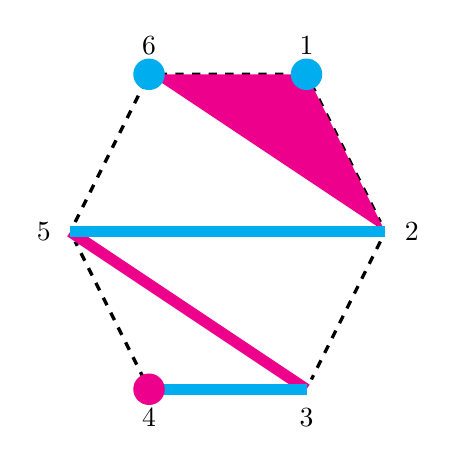
\begin{tikzpicture}[scale=1]
            \node [label = above : {$1$}] (1)
                at (4,5) {};
            \node [label = right : {$2$}] (2)
                at (5,3) {};
            \node [label = below : {$3$}] (3)
                at (4,1) {};
            \node [label = below : {$4$}] (4)
                at (2,1) {};
            \node [label = left : {$5$}]  (5)
                at (1,3) {};
            \node [label = above : {$6$}] (6)
                at (2,5) {};
            \draw [dashed][very thick]
            (1) -- (2) -- (3) -- (4)
                -- (5) -- (6) -- (1);
            \fill [color = magenta] (4,5) -- (5,3)
                -- (2,5) -- cycle;
            \draw [color = magenta][line width = 4pt] 
                (4,1) -- (1,3);
            \draw [color = cyan][line width = 4pt] 
                (4,1) -- (2,1);                
            \draw [color = cyan][line width = 4pt] 
                (5,3) -- (1,3);
            \fill [color=magenta] (2,1) circle (0.2);
            \fill [color=cyan] (4,5) circle (0.2);
            \fill [color=cyan] (2,5) circle (0.2);

          \end{tikzpicture}
    \end{center}
\end{example}

\subsection{Action of $\mathfrak{S}_n$ on partitions of 
$[n]$}

\begin{definition}[Action of $\mathfrak{S}_n$]
    The action of $\mathfrak{S}_n$ on a partition
    $P = \{B_1, \ldots, B_l\}$ of $[n]$ is defined by :\\
    \begin{itemize*}
        \item For each block $B_i = \{b_1, \ldots, b_k\}$ :
        $\sigma(Bi) =\{\sigma (b_1), \ldots, \sigma (b_k)\}$ \\
        \item When $P \in \mathcal{NC}_n$, we denote 
        $\rho = \sigma(P) =
            \{\sigma (B_1), \ldots, \sigma (B_l)\}$
    \end{itemize*}
\end{definition}

\begin{example}[$\sigma = 415362,
    P = \{\{1, 6\}, \{2, 3, 5\}, \{4\}\}$]
    ~\\
    $\sigma (P) = 
        \{\{1, 5, 6\}, \{2, 4\}, \{3\}\}$
        ~\\
    \begin{center}
        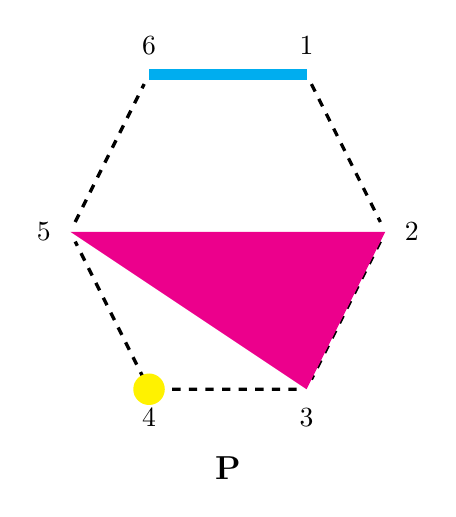
\begin{tikzpicture}[scale=1]
            \node at (3,0) {\large $\mathbf{P}$};
            \node [label = above : {$1$}] (1)
                at (4,5) {};
            \node [label = right : {$2$}] (2)
                at (5,3) {};
            \node [label = below : {$3$}] (3)
                at (4,1) {};
            \node [label = below : {$4$}] (4)
                at (2,1) {};
            \node [label = left : {$5$}]  (5)
                at (1,3) {};
            \node [label = above : {$6$}] (6)
                at (2,5) {};
            \draw [dashed][very thick]
            (1) -- (2) -- (3) -- (4)
                -- (5) -- (6) -- (1);
            \draw [color = cyan][line width = 4pt] 
                (4,5) -- (2,5);
            \fill [color = magenta] (5,3) -- (4,1)
                -- (1,3) -- cycle;
            \fill [color = yellow] (2,1) circle (0.2);
        \end{tikzpicture}
        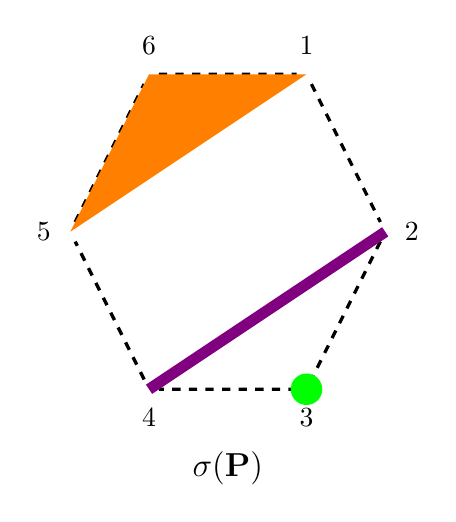
\begin{tikzpicture}[scale=1]
            \node at (3,0) {\large $\mathbf{\sigma(P)}$};
            \node [label = above : {$1$}] (1)
                at (4,5) {};
            \node [label = right : {$2$}] (2)
                at (5,3) {};
            \node [label = below : {$3$}] (3)
                at (4,1) {};
            \node [label = below : {$4$}] (4)
                at (2,1) {};
            \node [label = left : {$5$}]  (5)
                at (1,3) {};
            \node [label = above : {$6$}] (6)
                at (2,5) {};
            \draw [dashed][very thick]
            (1) -- (2) -- (3) -- (4)
                -- (5) -- (6) -- (1);
            \fill [color = orange] (4,5) -- (1,3)
                -- (2,5) -- cycle;
            \draw [color = violet][line width = 4pt] 
                (5,3) -- (2,1);
            \fill [color=green] (4,1) circle (0.2);

          \end{tikzpicture}
    \end{center}
\end{example}

\begin{rem}
    Note that $\mathcal{NC}_n$ is \emph{not} stable under
    the action of $\mathfrak{S}_n$.
    That is, even if $P$ is non-crossing, $\sigma (P)$ is 
    \emph{not} necessarily non-crossing.
\end{rem}

\begin{example}[Counter-example : $\sigma = 413562,
    P = \{\{1, 6\}, \{2, 3, 5\}, \{4\}\}$]
    $\sigma (P) = 
        \{\{1, 3, 6\}, \{2, 4\}, \{5\}\}$
        ~\\
    \begin{center}
        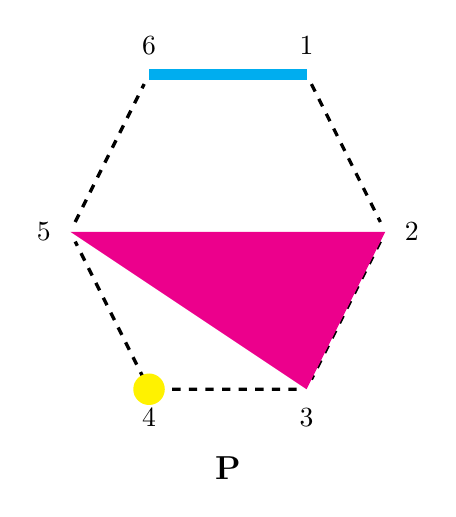
\begin{tikzpicture}[scale=1]
            \node at (3,0) {\large $\mathbf{P}$};
            \node [label = above : {$1$}] (1)
                at (4,5) {};
            \node [label = right : {$2$}] (2)
                at (5,3) {};
            \node [label = below : {$3$}] (3)
                at (4,1) {};
            \node [label = below : {$4$}] (4)
                at (2,1) {};
            \node [label = left : {$5$}]  (5)
                at (1,3) {};
            \node [label = above : {$6$}] (6)
                at (2,5) {};
            \draw [dashed][very thick]
            (1) -- (2) -- (3) -- (4)
                -- (5) -- (6) -- (1);
            \draw [color = cyan][line width = 4pt] 
                (4,5) -- (2,5);
            \fill [color = magenta] (5,3) -- (4,1)
                -- (1,3) -- cycle;
            \fill [color = yellow] (2,1) circle (0.2);
        \end{tikzpicture}
        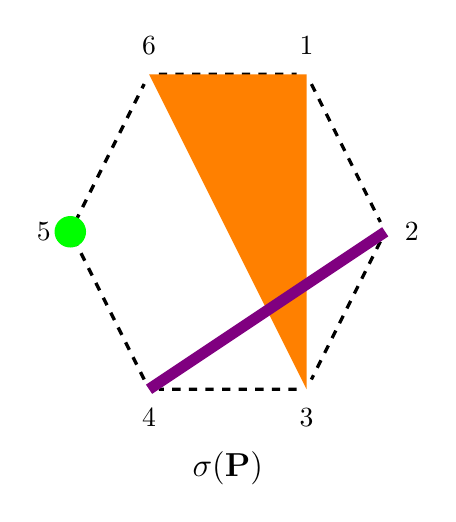
\begin{tikzpicture}[scale=1]
            \node at (3,0) {\large $\mathbf{\sigma (P)}$};
            \node [label = above : {$1$}] (1)
                at (4,5) {};
            \node [label = right : {$2$}] (2)
                at (5,3) {};
            \node [label = below : {$3$}] (3)
                at (4,1) {};
            \node [label = below : {$4$}] (4)
                at (2,1) {};
            \node [label = left : {$5$}]  (5)
                at (1,3) {};
            \node [label = above : {$6$}] (6)
                at (2,5) {};
            \draw [dashed][very thick]
            (1) -- (2) -- (3) -- (4)
                -- (5) -- (6) -- (1);
            \fill [color = orange] (4,5) -- (4,1)
                -- (2,5) -- cycle;
            \draw [color = violet][line width = 4pt] 
                (5,3) -- (2,1);
            \fill [color=green] (1,3) circle (0.2);
            
          \end{tikzpicture}
    \end{center}
\end{example}

\begin{definition}[Rotation]
    We define the \emph{rotation operator} $rot$ of
    $P \in \mathcal{NC}_n$ as $rot (P) = 
    (1\ 2\ 3\  \ldots \ n)(P) = 23 \ldots n1 (P)$.\\
    Conversely, we define $rot^{-1}$ of $P$ as
    $rot^{-1}(P) = (n\ n-1\ \ldots 3\ 2\ 1)(P) = 
    n12 \ldots n-1 (P)$.
\end{definition}

\begin{example}[$P = \{\{1, 6\}, \{2, 3, 5\}, \{4\}\}$]
    ~
    \begin{itemize}
        \item $rot (P) = \{\{1, 2\}, \{3, 4, 6\}, \{5\}\}$
        \item $rot^{-1}(P) = \{\{1, 2, 4\}, \{3\}, \{5, 6\}\}$
    \end{itemize}
    \begin{center}
    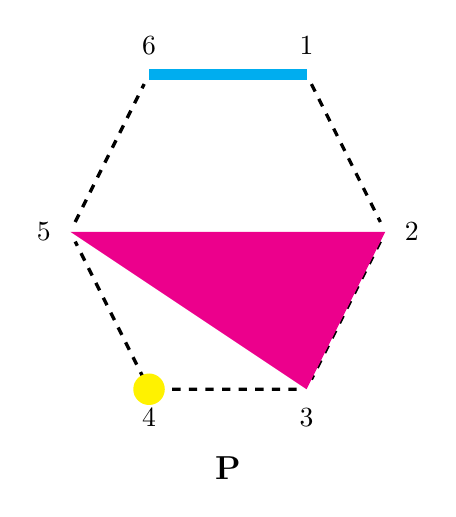
\begin{tikzpicture}[scale=1]
        \node at (3,0) {\large $\mathbf{P}$};
        \node [label = above : {$1$}] (1)
            at (4,5) {};
        \node [label = right : {$2$}] (2)
            at (5,3) {};
        \node [label = below : {$3$}] (3)
            at (4,1) {};
        \node [label = below : {$4$}] (4)
            at (2,1) {};
        \node [label = left : {$5$}]  (5)
            at (1,3) {};
        \node [label = above : {$6$}] (6)
            at (2,5) {};
        \draw [dashed][very thick]
        (1) -- (2) -- (3) -- (4)
            -- (5) -- (6) -- (1);
        \fill [color = magenta] (5,3) -- (4,1)
            -- (1,3) -- cycle;
        \draw [color = cyan][line width = 4pt] 
            (4,5) -- (2,5);
        \fill [color=yellow] (2,1) circle (0.2);
      \end{tikzpicture}
      ~\\
      ~\\

      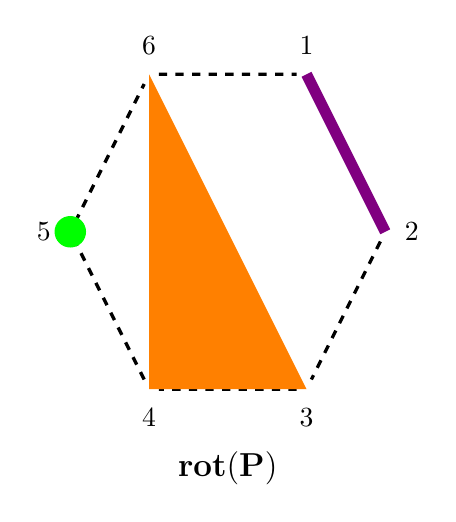
\begin{tikzpicture}[scale=1]
        \node at (3,0) {\large $\mathbf{rot(P)}$};
        \node [label = above : {$1$}] (1)
            at (4,5) {};
        \node [label = right : {$2$}] (2)
            at (5,3) {};
        \node [label = below : {$3$}] (3)
            at (4,1) {};
        \node [label = below : {$4$}] (4)
            at (2,1) {};
        \node [label = left : {$5$}]  (5)
            at (1,3) {};
        \node [label = above : {$6$}] (6)
            at (2,5) {};
        \draw [dashed][very thick]
        (1) -- (2) -- (3) -- (4)
            -- (5) -- (6) -- (1);
        \fill [color = orange] (4,1) -- (2,1)
            -- (2,5) -- cycle;
        \draw [color = violet][line width = 4pt] 
            (4,5) -- (5,3);
        \fill [color=green] (1,3) circle (0.2);    
      \end{tikzpicture}
      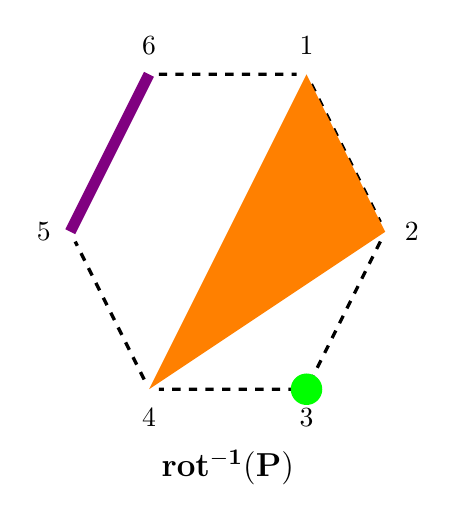
\begin{tikzpicture}[scale=1]
        \node at (3,0) {\large $\mathbf{rot^{-1}(P)}$};
        \node [label = above : {$1$}] (1)
            at (4,5) {};
        \node [label = right : {$2$}] (2)
            at (5,3) {};
        \node [label = below : {$3$}] (3)
            at (4,1) {};
        \node [label = below : {$4$}] (4)
            at (2,1) {};
        \node [label = left : {$5$}]  (5)
            at (1,3) {};
        \node [label = above : {$6$}] (6)
            at (2,5) {};
        \draw [dashed][very thick]
        (1) -- (2) -- (3) -- (4)
            -- (5) -- (6) -- (1);
        \fill [color = orange] (4,5) -- (5,3)
            -- (2,1) -- cycle;
        \draw [color = violet][line width = 4pt] 
            (1,3) -- (2,5);
        \fill [color=green] (4,1) circle (0.2);    
      \end{tikzpicture}
    \end{center}
\end{example}

\begin{rem}
    ~
    \begin{itemize}
        \item $rot (rot^{-1}(P)) = rot^{-1}(rot(P)) = P$
        \item $rot(P)$ and $rot^{-1}(P)$ are always
            non-crossing partitions.
        \item If $P \in \mathcal{NC}_n$, then $rot^n(P) =
            rot^{-n}(P) = P$.
    \end{itemize}
\end{rem}

\begin{prop}
    $K (K (P)) = rot^{-1} (P)$.
\end{prop}

\begin{example}[$P = \{\{1, 6\}, \{2, 3, 5\}, \{4\}\}$]
    ~
    \begin{center}
        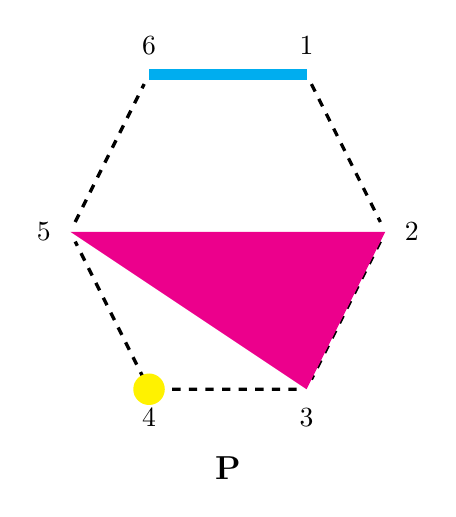
\begin{tikzpicture}[scale=1]
            \node at (3,0) {\large $\mathbf{P}$};
            \node [label = above : {$1$}] (1)
                at (4,5) {};
            \node [label = right : {$2$}] (2)
                at (5,3) {};
            \node [label = below : {$3$}] (3)
                at (4,1) {};
            \node [label = below : {$4$}] (4)
                at (2,1) {};
            \node [label = left : {$5$}]  (5)
                at (1,3) {};
            \node [label = above : {$6$}] (6)
                at (2,5) {};
            \draw [dashed][very thick]
            (1) -- (2) -- (3) -- (4)
                -- (5) -- (6) -- (1);
            \fill [color = magenta] (5,3) -- (4,1)
                -- (1,3) -- cycle;
            \draw [color = cyan][line width = 4pt] 
                (4,5) -- (2,5);
            \fill [color=yellow] (2,1) circle (0.2);
          \end{tikzpicture}
          ~\\
          ~\\
    
          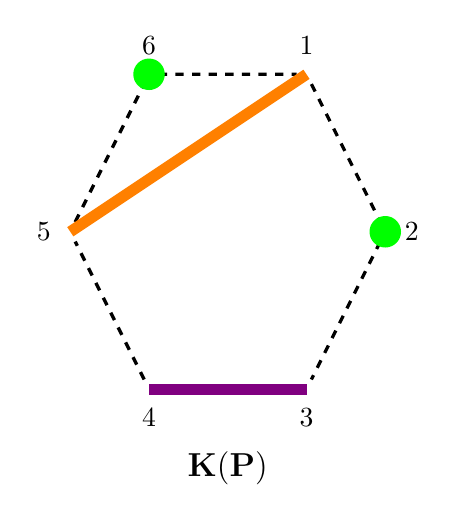
\begin{tikzpicture}[scale=1]
            \node at (3,0) {\large $\mathbf{K(P)}$};
            \node [label = above : {$1$}] (1)
                at (4,5) {};
            \node [label = right : {$2$}] (2)
                at (5,3) {};
            \node [label = below : {$3$}] (3)
                at (4,1) {};
            \node [label = below : {$4$}] (4)
                at (2,1) {};
            \node [label = left : {$5$}]  (5)
                at (1,3) {};
            \node [label = above : {$6$}] (6)
                at (2,5) {};
            \draw [dashed][very thick]
            (1) -- (2) -- (3) -- (4)
                -- (5) -- (6) -- (1);
            \draw [color = orange][line width = 4pt] 
                (4,5) -- (1,3);            
            \draw [color = violet][line width = 4pt] 
                (4,1) -- (2,1);
            \fill [color=green] (5,3) circle (0.2); 
            \fill [color=green] (2,5) circle (0.2);   
          \end{tikzpicture}
          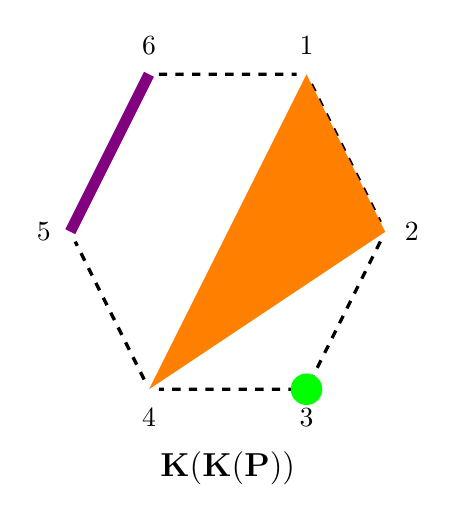
\begin{tikzpicture}[scale=1]
            \node at (3,0) {\large $\mathbf{K(K(P))}$};
            \node [label = above : {$1$}] (1)
                at (4,5) {};
            \node [label = right : {$2$}] (2)
                at (5,3) {};
            \node [label = below : {$3$}] (3)
                at (4,1) {};
            \node [label = below : {$4$}] (4)
                at (2,1) {};
            \node [label = left : {$5$}]  (5)
                at (1,3) {};
            \node [label = above : {$6$}] (6)
                at (2,5) {};
            \draw [dashed][very thick]
            (1) -- (2) -- (3) -- (4)
                -- (5) -- (6) -- (1);
            \fill [color = orange] (4,5) -- (5,3)
                -- (2,1) -- cycle;
            \draw [color = violet][line width = 4pt] 
                (1,3) -- (2,5);
            \fill [color=green] (4,1) circle (0.2);    
          \end{tikzpicture}
        \end{center}
\end{example}